\exercicio{}

O método geométrico de corte e colagem aparece no manual\parencite[pág. 77-78]{Estrada2000} como uma
hipótese de Neugebauer sobre qual os babilónios aproximaram o valor de $\sqrt{2}$.
Este método pode ser utilizado para iterativamente calcular a raíz de qualquer $N \in \mathbb{N}$.

\vspace{0.25cm}

\noindent
Consideremos:
\begin{itemize}
	\item $N\in \mathbb{N}$, o número pelo qual pretendemos calcular a raíz quadrada;
	\item $x_0 \in \mathbb{N}$ é uma estimativa por excesso;
	\item $y_0 \in \mathbb{N}$ é uma estimativa por defeito;
	\item $N = x_0 y_0$
\end{itemize}

\noindent
Do manual\parencite[pág. 77]{Estrada2000}, tem-se as seguintes relações de recorrência, por
Neugebauer:

\begin{align*}
	\begin{cases}
		x_{n + 1} = \frac{x_n + y_n}{2}\\
		y_{n + 1} = \frac{N}{x_{n+1}}
	\end{cases}
	\implies N = x_n \cdot y_n
\end{align*}

\noindent
De modo a criar um critério de paragem eficaz, comecemos por provar quer $y_n \leq x_n \leq N,
\forall n \in \mathbb{N}$.

\begin{enumerate}
	\item Caso base: para $n = 0$, temos por definição que $x_0 \geq y_0$.
	\item Supomos que: $x_n \geq y_n$(Hipótese de Indução)
	\item Pretendemos provar que: $x_{n+1} \geq y_{n+1}$ (Tese de Indução)
	\item Verifiquemos se $x_{n + 1} \geq y_{n + 1}$, com base na Hipótese de Indução:
		\begin{align*}
			x_{n + 1} = \frac{x_n + y_n}{2} &\geq \frac{N}{x_{n + 1}} = y_{n +1} \\ 
			\iff x_n^2 + y_nx_n &\geq 2x_ny_n\\
			\iff x_n^2 &\geq y_nx_n\\
			\iff x_n &\geq y_n
		\end{align*}
		Damos deste modo o passo de indução $x_n > y_n$ de indução, podemos concluir que $x_{n +1}
		\geq y_{n + 1}$.
\end{enumerate}

Os digramas da figura na página seguinte descreve o processo de iteração geométrica pelo método de corte e
colagem. Deste diagrama também derivamos a fórmula de erro.

A partir do diagrama (c) temos que a fórmula de erro para uma dada iteração $n$, porque
$x_n \geq y_n$,  é majorado por:

\begin{align*}
	\varepsilon_n = x_n - y_n
\end{align*}


\clearpage
\begin{figure}[ht!]
	\centering
	\begin{subfigure}[b]{0.3\textwidth}
	\centering
	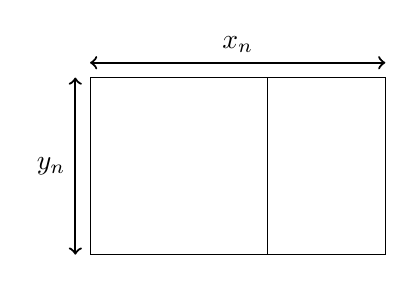
\begin{tikzpicture}[scale=0.75]
	\draw (0, 0) rectangle (5, 3);
	\draw (3, 0) -- (3, 3);
	\node[left] at (-0.25, 1.5) {$y_n$};
	\node[above] at (2.5, 3.25) {$x_n$};
	\draw[thick,<->] (0, 3.25) -- (5, 3.25);
	\draw[thick,<->] (-0.25, 0) -- (-0.25, 3);
\end{tikzpicture}

	\caption{}
	\end{subfigure}
	\begin{subfigure}[b]{0.30\textwidth}
	\centering
	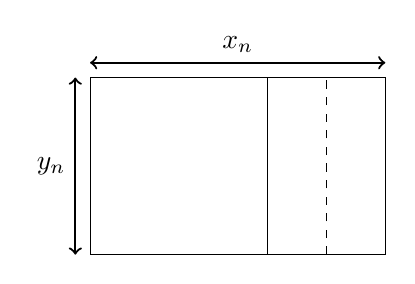
\begin{tikzpicture}[scale=0.75]
	\draw (0, 0) rectangle (5, 3);
	\draw (3, 0) -- (3, 3);
	\draw[dashed] (4, 0) -- (4, 3);
	\node[left] at (-0.25, 1.5) {$y_n$};
	\node[above] at (2.5, 3.25) {$x_n$};
	\draw[thick,<->] (0, 3.25) -- (5, 3.25);
	\draw[thick,<->] (-0.25, 0) -- (-0.25, 3);
\end{tikzpicture}

	\caption{}
	\end{subfigure}
	\begin{subfigure}[b]{0.30\textwidth}
	\centering
	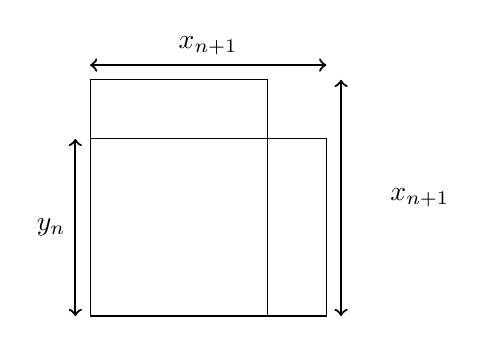
\begin{tikzpicture}[scale=0.75]
	\draw (0, 0) rectangle (4, 3);
	\draw (0, 3) rectangle (3, 4);
	\draw (3, 0) -- (3, 3);
	\node[left] at (-0.25, 1.5) {$y_n$};
	\node[above] at (2, 4.25) {$x_{n + 1}$};
	\node[left] at (6.25, 2) {$x_{n + 1}$};
	\draw[thick,<->] (0, 4.25) -- (4, 4.25);
	\draw[thick,<->] (-0.25, 0) -- (-0.25, 3);
	\draw[thick,<->] (4.25, 0) -- (4.25, 4);
\end{tikzpicture}

	\caption{}
	\end{subfigure}

	\bigskip

	\begin{subfigure}{0.4\textwidth}
	\centering
	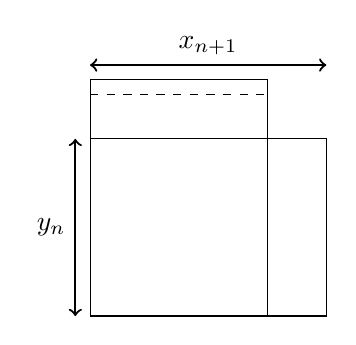
\begin{tikzpicture}[scale=0.75]
	\draw (0, 0) rectangle (4, 3);
	\draw (0, 3) rectangle (3, 4);
	\draw[dashed] (0, 15/4) -- (3, 15/4);
	\draw (3, 0) -- (3, 3);
	\node[left] at (-0.25, 1.5) {$y_n$};
	\node[above] at (2, 4.25) {$x_{n + 1}$};
	\draw[thick,<->] (0, 4.25) -- (4, 4.25);
	\draw[thick,<->] (-0.25, 0) -- (-0.25, 3);
\end{tikzpicture}

	\caption{}
	\end{subfigure}
	\begin{subfigure}{0.4\textwidth}
	\centering
	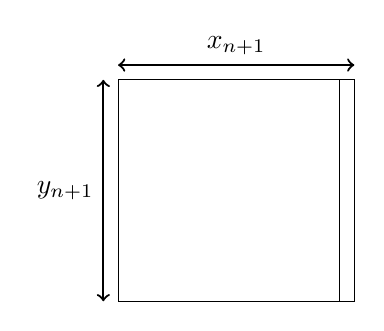
\begin{tikzpicture}[scale=0.75]
	\draw (0, 0) rectangle (4, 15/4);
	\draw (15/4, 0) -- (15/4, 15/4);
	\node[left] at (-0.25, 15/8) {$y_{n + 1}$};
	\node[above] at (2, 4) {$x_{n + 1}$};
	\draw[thick,<->] (0, 4) -- (4, 4);
	\draw[thick,<->] (-0.25, 0) -- (-0.25, 15/4);
\end{tikzpicture}

	\caption{}
	\end{subfigure}
	\caption{Processo iterativo de cálculo de aproximações de $\sqrt{N}$}%
\end{figure}


\paragraph{\underline{Cálculo $\sqrt{15}$, com $\varepsilon \leq 10^{-5}$}}
\hfill

\paragraph{Resposta} $\sqrt{15} = \frac{7440}{1921} \pm \frac{1}{962816}$

\begin{table}[h]
	\centering
	\label{tab:raiz-15-iteracoes}
	\begin{tabular}{|r|l|l|l|}
		\hline
		$i$ & $x_i$ & $y_i$ & $\varepsilon$\\
		\hline
		\csvreader[
			no head,
			late after line = \\\hline
		]{data/ex2.csv} {}{
			\csvcoli & \csvcolii &\csvcoliii &\csvcoliv
		}
	\end{tabular}
	\caption{Iterações do algoritmo}
\end{table}

\begin{align*}
	N
	&= 15 = 5 \cdot 3\\
	&\begin{cases}
		x_0 &= 5\\
		y_0 &= 3\\
		e_0 &= 2
	\end{cases}\\
	&\begin{cases}
		x_1 &= \frac{x_0 + y_0}{2} = 4\\
		y_1 &= \frac{2N}{x_0 + y_0} = \frac{15}{4}\\
		e_1 &= \frac{1}{4}
	\end{cases}\\
	&\begin{cases}
		x_2 &= \frac{x_1 + y_1}{2} = \frac{31}{8}\\
		y_2 &= \frac{2N}{x_1 + y_1} = \frac{120}{31}\\
		e_2 &= \frac{1}{248}
	\end{cases}\\
	&\begin{cases}
		x_3 &= \frac{x_2 + y_2}{2} = \frac{1921}{496}\\
		y_3 &= \frac{2N}{x_2 + y_2} = \frac{7440}{1921}\\
		e_2 &= \frac{1}{952816}
	\end{cases}
\end{align*}

